\section{Confidentiality Policies}

Una politica di riservatezza, chiamata anche “information flow policy”,
impedisce la divulgazione
non autorizzata di informazioni. Il suo obiettivo è quello di specificare quali
dati devono essere
protetti e da chi o da che cosa vanno protetti. In poche parole, indicano un
insieme di principi e
regole che definiscono i possibili accessi al sistema.

Distinguiamo tra:

\begin{itemize}
    \item \textbf{Oggetti:} una qualunque entità passiva che necessita di
          essere protetta;
    \item \textbf{Soggetti:} una qualunque entità attiva che può manipolare
          gli oggetti (persone o processi).
\end{itemize}

Un modello di sicurezza definisce i soggetti, gli oggetti ai quali i soggetti
hanno accesso ed i diritti
di accesso, che non sono altro che le operazioni con le quali è possibile
operare. Un soggetto può
avere diritti di accesso sia per gli oggetti che per altri soggetti.
Esistono due tipi di modelli di sicurezza:
\begin{itemize}
    \item \textit{Discretionary access control} (\textbf{DAC}): meccanismo
          attraverso il quale gli utenti possono
          liberamente decidere di garantire o revocare l'accesso a determinati
          oggetti.
          \begin{itemize}
              \item Gli utenti amministrano i dati che possiedono (vengono
                    detti proprietari);
              \item Il proprietario può autorizzare altri utenti all'accesso;
              \item Il proprietario può definire il tipo di accesso da
                    concedere agli altri;
              \item Accessi selettivi.
          \end{itemize}
    \item \textit{Mandatory access control} (\textbf{MAC}): meccanismo
          attraverso il quale le decisioni di accesso
          sono basate su delle etichette che contengono informazioni
          rilevanti alla sicurezza di un
          oggetto. Questo metodo fornisce l'accesso alla risorsa in base al
          livello di autorizzazione dell'utente.
          \begin{itemize}
              \item Classificazione dei dati (livelli di sensibilità);
              \item Classificazione dei soggetti (autorizzazione);
              \item Classe di sicurezza <componente gerarchica, insiemi di
                    categoria>;
              \item Ordinamento (parziale) tra le classi di sicurezza;
              \item I meccanismi di sicurezza devono garantire che tutti i
                    soggetti abbiano accesso solo
                    ai dati per cui possiedono le autorizzazioni appropriate;
              \item Non si possono propagare privilegi.
          \end{itemize}
\end{itemize}

\subsection{Modello Bell-LaPadula}
È un modello tipico \textbf{MAC}. Fu proposto da Bell-LaPadula nel 1976 con lo scopo di
rafforzare i
controlli ai possibili accessi alle applicazioni militari (corrisponde, infatti,
alle classificazioni
stile-militare). Viene anche chiamato modello “\textit{a multi-livelli}”.
Nelle applicazioni i soggetti e gli oggetti vengono partizionati in differenti
livelli di sicurezza. Un
soggetto può solo accedere ad oggetti a certi livelli, i quali dipendono
strettamente dal loro
livello di sicurezza. Per esempio, i seguenti sono due tipici specificazioni di
accessi: “una persona
\verb|UNCLASSIFIED| non può leggere informazioni a livello \verb|CONFIDENTIAL|” e
“informazioni \verb|TOP SECRET| non possono essere scritte in files di livello
\verb|UNCLASSIFIED|”.
Gli oggetti sono classificati in 4 diversi livelli di sensibilità, cioè di
confidentiality. Ciascun oggetto
può essere associato a uno o più livelli, detti compartments.
Ad ogni soggetto, invece, viene associata una “\textit{clearance}” ovvero
un'autorizzazione. Una
clearance non è altro che una coppia del tipo \verb|<rank, compartments>|
dove \verb|rank| è il massimo livello di sensibilità dell'informazione a cui
il soggetto ha accesso; \verb|compartment| indica i comparti a
cui il soggetto può accedere.
A tutte le entità vengono assegnati dei livelli di sicurezza. In particolare:

\begin{itemize}
    \item Un soggetto S possiede “\textit{security clearance}” \(L(S)=l_s\);
    \item Un oggetto O possiede “\textit{security classification}” \(L(O)=l_o\);
\end{itemize}

Per ogni classificazione di sicurezza \(l_i, \ i=0,...,k-1 \ con \ l_i<l_i+1\),
quindi i livelli di sicurezza sono
disposti in ordine lineare.
Il tipo più semplice di classificazione della confidenzialità è un insieme di
autorizzazioni poste in
gerarchia: \verb|Top secret > Secret > Confidential > Unclassified|.
Il modello definisce due regole obbligatorie del controllo accessi (MAC):
\begin{itemize}
    \item \textbf{Simple Security Condition:} S può leggere O se e solo se
          \(l_o \le l_s\) e S ha discrezione
          nell'accesso in lettura a O. Questa regola viene anche detta “No Read Up”
          e impedisce ai
          soggetti di leggere oggetti a livelli superiori. Il proprietario può
          aggiungere anche dei diritti di
          tipo DAC, ovvero può restringere ulteriormente l'accesso.
    \item \textbf{* Property} (Star property): S può scrivere su O se e solo
          se \(l_s \le l_o\) e S ha discrezione
          nell'accesso alla scrittura su O. La regola è anche detta “No Write Down”
          e impedisce ai
          soggetti di scrivere su oggetti di livello inferiore. Questo perché se no
          un utente potrebbe declassificare
          informazioni o oggetti scrivendoli all'interno di oggetti con grado di
          classificazione inferiore.
\end{itemize}

Si potrebbe estendere il modello addizionando un gruppo di categorie per ogni
classificazione di
sicurezza. Ogni categoria descrive un tipo di informazioni.
Tali categorie risultano dal principio del “Need To know”: limito l'accesso alle
sole informazioni per
le quali l'utente ha necessità di accedere.

\paragraph{Esempio:}
CATEGORIE \(\rightarrow\) Alpha, Beta e Gamma.
Ogni soggetto ha un'autorizzazione ad un determinato livello di sicurezza e può
accedere anche
ad alcuni dei livelli inferiori.

\begin{figure}[H]
    \centering
    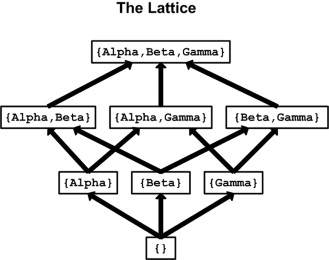
\includegraphics[width=8cm, keepaspectratio]{capitoli/policy/imgs/Lattuce.jpg}
\end{figure}

\subsection{Multilevel Security}
Il concetto viene trattato per la prima volta nel “Red Book”nel 1987.
La sicurezza multilivello o più livelli di sicurezza (\textbf{MLS}) è
l'applicazione di un sistema di computer
per elaborare le informazioni con incompatibili classificazioni (cioè, a diversi
livelli di sicurezza),
consentire l'accesso da parte di utenti con diversi spazi di sicurezza e le
esigenze di sapere (need
to know) e impedire agli utenti di ottenere l'accesso alle informazioni per
le quali non hanno
l'autorizzazione.
La sicurezza multilivello viene implementata in ambiti particolari, dove è
necessario un controllo
obbligatorio degli accessi, per assicurare che le politiche di sicurezza siano
garantite dal sistema.
L'ente definisce delle regole in merito a chi può accedere e anche a che cosa;
queste regole non
possono essere modificate dai singoli utenti.
I sistemi MLS ci assicurano diversi livelli di sicurezza L che definiscono la
classificazione dei
soggetti (processi) e degli oggetti. I livelli di affidabilità, cioè di
“assurance”, vengono stabiliti in
base a vari criteri di valutazione:
\[
    (worst) \ D<C1<C2<C3<B1<B2<B3<A1 \ (best)
\]
In base ai dati e alle circostanze possono essere richiesti livelli più o meno
elevati. Solitamente, in
presenza di un solo livello, è sufficiente una macchina del tipo C2 o C3. Da B1
in poi, invece, si
possono gestire efficacemente informazioni su livelli multipli.
\begin{center}
    \begin{tabular}{ |c|c| }
        \hline
        \textbf{System Stores}   & \textbf{Minimum Assurance} \\
        \hline
        TopSecret + Unclassified & B3                         \\
        \hline
        TopSecret + Secret       & B2                         \\
        \hline
        Secret + Unclassified    & B1                         \\
        \hline
    \end{tabular}
\end{center}
TopSecret+Unclassified rappresentano in realtà 3 livelli, insieme al Secret.
Attaccare una macchina B3 costa certamente di più che attaccare B1 o B2.

\subsubsection{Channel Cascade Attacks}

Prendiamo in esame la seguente immagine:
\begin{figure}[H]
    \centering
    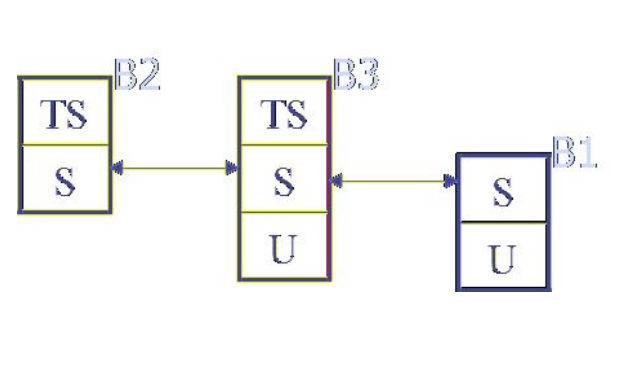
\includegraphics[width=8cm, keepaspectratio]{capitoli/policy/imgs/cascade1.png}
\end{figure}
I livelli di sicurezza delle macchine sono B1, B2 e B3. Lo
sforzo (l'effort) viene effettuato da un attaccante, il quale
cerca di penetrare una macchina con un determinato livello
di sicurezza.
Il “\textbf{cascade attack}” si ha quando una sola macchina viene attaccata ad
un certo livello, ma anche
le altre vengono coinvolte conseguentemente.
L'informazione tra i sistemi è condivisa, quindi può fluire tra le macchine.
Nell'esempio, infatti, sono
tutte collegate a livello S. Grazie all'effort su B2 si riesce a portare
l'informazione da TS a U, che
equivale a dire di aver buttato giù un sistema B3. Quindi, a partire da B2,
si riesce a buttar giù
anche B1 e B3.
Si dice “attacco a cascata” perché grazie ad uno sforzo relativamente piccolo
(nel nostro caso
effettuato su B2) si possono attaccare anche sistemi più grandi e sicuri,
poiché sono interconnessi.
In generale quindi, se l'attacco ha successo, il livello di segretezza può
essere abbassato da
TopSecret a Secret, fino a Unclassified.
Si ha un “cascading attack” se esiste un “cascading path”, ovvero un cammino
tra sistemi che
costa meno dello sforzo necessario a rompere i singoli sistemi.
Ricordiamo che eliminare i cascade path è un problema che rientra in NP.

\paragraph{Come eliminate il Cascade Path}
\begin{itemize}
    \item  Si possono disconnettere le macchine. Più c'è condivisione,
          più si alza la possibilità di
          avere cascading path;
    \item  Mettere in comunicazione le macchine a livelli diversi;
    \item  Definire i flussi consentiti (ognuno avrà uno specifico costo).
\end{itemize}
Il seguente non è un cascading path (non va bene perché dovremmo
rompere un sistema B3. L'effort è uguale all'attacco, non c'è il
guadagno).
\begin{figure}[H]
    \centering
    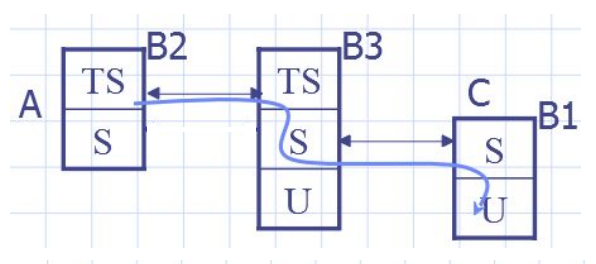
\includegraphics[width=8cm, keepaspectratio]{capitoli/policy/imgs/cascade3.png}
\end{figure}
Questo invece è un cascading path (quando il livello dell'attacco è più
grande dello sforzo).
\begin{figure}[H]
    \centering
    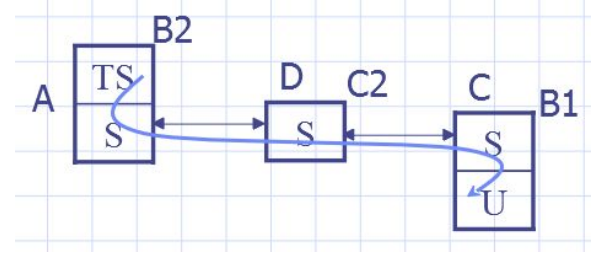
\includegraphics[width=8cm, keepaspectratio]{capitoli/policy/imgs/cascade2.png}
\end{figure}

\subsection{Secure Interoperation}

\begin{figure}[H]
    \centering
    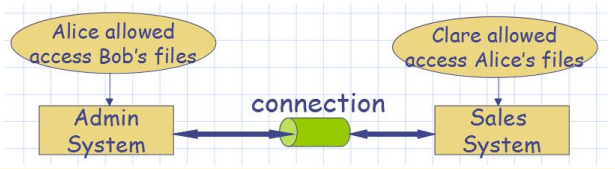
\includegraphics[width=10cm, keepaspectratio]{capitoli/policy/imgs/secure_interoperation.png}
\end{figure}

Supponiamo di avere due sistemi all'interno ad un'azienda, uno per le Vendite e
uno per
l'Amministrazione. Ognuno ha la propria policy che chiaramente definisce i
diritti degli utenti.
Alice lavora su entrambi i sistemi e vorrebbe che i filesystem venissero
connessi (I sistemi sono
sicuri individualmente). Se ciò avvenisse, allora anche Clare avrebbe accesso
ai file dell'Admin
System. Ciò rappresenta a tutti gli effetti un attacco al sistema.

Le possibili soluzioni sono:

\begin{itemize}
    \item Togliere a Clare l'accesso ai file di Alice;
    \item togliere ad Alice l'accesso ai file di Bob.
\end{itemize}

In generale quindi è necessario riconfigurare il sistema in modo da eliminare
alcune connessioni e
di conseguenza ridurre i diritti degli utenti.

\subsection{Access Interoperation}

\begin{figure}[H]
    \centering
    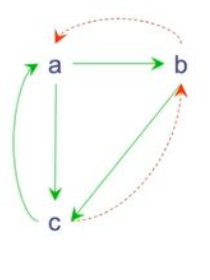
\includegraphics[width=4cm, keepaspectratio]{capitoli/policy/imgs/access_interoperation.png}
\end{figure}

Consideriamo la figura precedente che ci mostra una policy (rappresentata dalle
linee verdi) la quale definisce i seguenti accessi.
L'accesso da \verb|A| a \verb|C| potrebbe essere ottenuto per transitività
passando per \verb|B|.
Stesso discorso vale per \verb|C| e \verb|B|: da \verb|C| si può arrivare a
\verb|B| tramite \verb|A|. Ma il fatto che
da \verb|C| si possa raggiungere \verb|B| viola la policy, perché questo accesso
non è definito in realtà. \'{E} necessario quindi riconfigurare il sistema.
Eventuali soluzioni potrebbero essere:
\begin{itemize}
    \item Esplicitare i flussi, quindi ciò che è effettivamente permesso e
          cosa non lo
          è (ovvero aggiungere anche le linee rosse);
    \item Esplicitare soltanto ciò che è vietato (linee rosse) e quindi il
          resto è default permit;
    \item Esplicitare soltanto ciò che è permesso (linee verdi) e quindi il
          resto è default deny.
\end{itemize}
Va ricordato che la riconfigurazione deve essere safe: ciò che viene stabilito
con la nuova
configurazione deve
essere un sottoinsieme di ciò che era permesso anche prima: non dobbiamo andare
ad escludere per errore flussi già esistenti. La policy deve essere rispettata
sempre, anche dopo la riconfigurazione.

\subsection{Secure Reconfiguration}

Supponiamo di avere due differenti policy, corrispondenti a due diversi sistemi
che devono però
interoperare. Unire le due policy potrebbe non essere così semplice, in quanto
potrebbero
verificarsi dei conflitti.
A questo punto è necessario capire a cosa dare priorità, se a ciò che è permesso
o a ciò che non lo è. Solitamente si dà priorità al default deny, altrimenti
non ci sarebbe garanzia del fatto che il sistema sia ancora safe.

\begin{figure}[H]
    \centering
    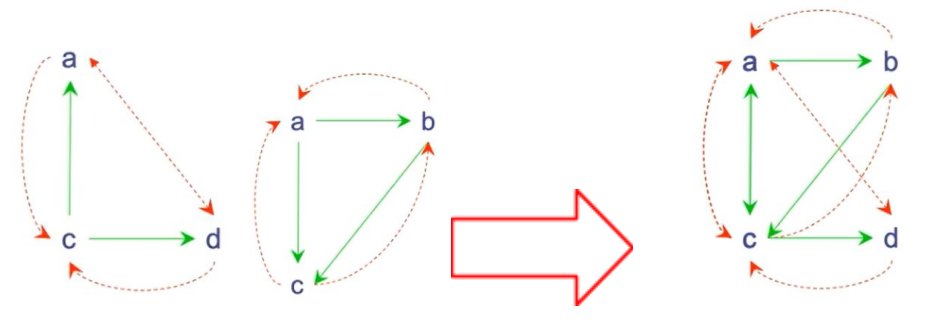
\includegraphics[width=10cm, keepaspectratio]{capitoli/policy/imgs/secure_recognition.png}
\end{figure}

Una volta esplicitato cosa è vietato, si può definire cosa è invece permesso,
assicurando il fatto
che non ci sia alcuna transitività.
Il nuovo schema della policy deve essere proiettato sui sistemi a cui è
destinato per verificare che
non si presentino comunicazioni non corrette.

\begin{figure}[H]
    \centering
    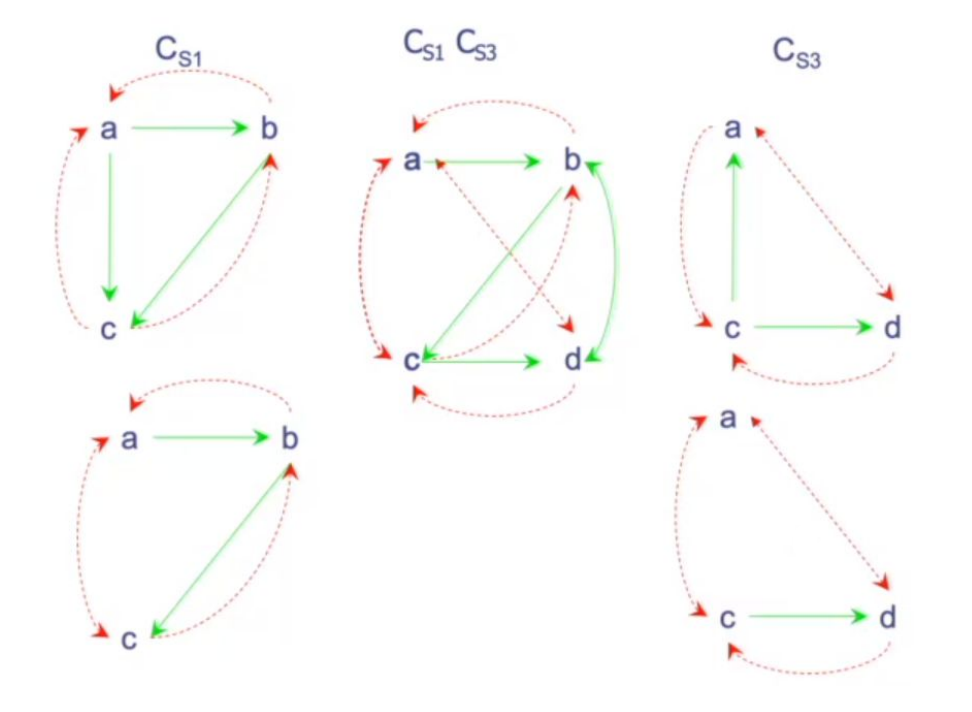
\includegraphics[width=12cm, keepaspectratio]{capitoli/policy/imgs/secure_regognition2.png}
\end{figure}
